\documentclass[conference]{IEEEtran}
\usepackage{lipsum} %<---- For dummy text
\usepackage{xcolor}% you could also use the color package
\usepackage{colortbl}
\usepackage{marvosym}
\usepackage{txfonts}
\usepackage{graphicx}
\usepackage{footnote}
\usepackage{epstopdf} %%package to overcome problem with eps in pdf files
\usepackage{natbib}
\usepackage{url}
\usepackage{float}


\title{Awsseract: Distributed OCR processing service  \\  {\large IN4392 Cloud Computing} }

\author{
\IEEEauthorblockN{Joseph Hejderup}
\IEEEauthorblockA{4245210 \\ Delft University of Technology \\
The Netherlands \\
\texttt{joseph.hejderup@gmail.com}}\\ \\[0.3cm]
\IEEEauthorblockN{Bogdan Ghit}
\IEEEauthorblockA{Lab Assistance \\ Parallel and Distributed Systems Group
 \\ Delft University of Technology \\
The Netherlands \\
\texttt{B.I.Ghit@tudelft.nl}}\\ 
\and
\IEEEauthorblockN{Wing Lung Ngai}
\IEEEauthorblockA{1511483 \\ Delft University of Technology \\
The Netherlands \\
\texttt{winglung.ngai@gmail.com}}\\[0.7cm]
\IEEEauthorblockN{Alexandru Iosup}
\IEEEauthorblockA{Course Instructor \\ Parallel and Distributed Systems Group
 \\ Delft University of Technology \\
The Netherlands \\
\texttt{A.Iosup@tudelft.nl}}\\ 
\and
\IEEEauthorblockN{Wenbo Zhao}
\IEEEauthorblockA{4123379 \\ Delft University of Technology \\
The Netherlands \\
  \texttt{W.Zhao@student.tudelft.nl}}\\[0.7cm]
\IEEEauthorblockN{Dick Epema}
\IEEEauthorblockA{Course Instructor \\ Parallel and Distributed Systems Group
 \\ Delft University of Technology \\
The Netherlands \\
\texttt{D.H.J.Epema@tudelft.nl}}\\ 

}

\begin{document}


\maketitle



\begin{abstract}
Awsseract, a distributed implementation of the popular open-course Tesseract OCR engine for extracting text elements from scanned images. Awsseract is the a cloud-based implementation for IaaS platforms and modeled after the actor model and work-stealing pattern to achieve high scalability and effective load-balancing. ---PROVIDE THE RESULT INFO HERE---


\end{abstract}

\section{Introduction}\label{sec:intro}
\noindent

% TODO: References and section numbers
WantCloud BV, an IT consultancy firm specialized in development and hosting of web application, is seeking new business opportunities to expand their consultancy services with cloud-based applications. WantCloud is currently experiencing an increasing resource demand in their on-premise datacenters from their clients while the resource utilization rate of their datacenters is very low. This has lead to clients complaining about poor scalability (e.g. clients losing money due to sudden high end-user demand) and that WantCloud does not fulfill its obligations in the SLA conditions. In order to be a competitive contender in the market, WantCloud is considering to migrate to a Hybrid solution where the on-premise datacenter and an IaaS provider will meet the increased resource demand and offer better elasticity and Quality of Service (QoS). 

 
IaaS (Infrastructure as a Service) is a provisioning model in which a third-party organization provide computation, storage and networking resources on demand, in a pay-per-use fashion \cite{LectureCC}. IaaS providers emphasize the value of elasticity, in terms of scalability, low maintenance costs, good performance and reliability. WantCloud BV is particularly interested in the concepts of load variability support and minimum up-front investments. Amazon is the largest commercial IaaS provider, offering cloud services such as Simple Storage Service (S3) and Elastic Compute Cloud (EC2) under the umbrella name ”Amazon Web Services (AWS)”. WantCloud would like to investigate the feasibility of using Amazon EC2 as a potential candidate in their expansion.
 
For this purpose, Awsseract is a prototype application built on the top of Amazon EC2 \cite{amazon}, developed to assess the usability and the performance of the IaaS platform. Its actual application is an image-processing web-service that extracts textual fields from images by using the popular Google-owned Tesseract engine. Tesseract is an open-source optical character recognition (OCR) engine originally developed at Hewlett Packard Labs in 1985 but was open-sourced in 2006 \cite{tess}.  The current version is 3.02 and supports multiple image formats (using Leptonica) and recognition of over 40 languages such as Dutch, Chinese or Arabic.

Awsseract is modeled in a distributed-fashion to support fault-tolerance, scalability with high responsiveness. Functional programming languages and concurrency models such as the Actor Model are emerging as a more concise and mathematical way to reason about programs. Therefore the Scala programming language is used to develop the fundamental core structure of Assersact, leveraging the Akka framework for a distributed Actor-based system and the Play! Framework for the front-end design.  The Scala programming language and the use of the Actor Model is emerging as modern tools for building software for cloud computing architecture. One of the main reasons is that Scala has a concise syntax and relies heavily on functional principles to reduce the complexity of system. Unlike the Shared Memory Model used in Java of which the shared mutable states often lead to race conditions, blocking and deadlocks, the Actor model is an immutable model that is asynchronous, race-free and with non-blocking queue using a message-passing model \cite{akka}.
        
The main goal of this project is to show how an image-processing problem can be highly scalable in terms of large user demand without compromising the responsiveness and interactivity of the service. 

The remainder of report is as follows: Section~\ref{sec:bg} contains a brief description and a requirements analysis of the Awsseract service. The system architecture and implementation details are explained in Section~\ref{sec:sysdesign}. Finally, Section~\ref{sec:experiment} contains the performance evaluation of Awsseract service, followed by conclusion and our recommendations for WantCloud. 

\section{Application Requirements}\label{sec:bg}
\noindent
Awsseract has to conform with the business objectives of WantCloud by assessing the implications and possibilities of leveraging computing power from an IaaS supplier. Therefore, Awsseract should have distributed properties such as elasticity, monitoring, reliability, etc. Moreover, it should be able to set limitation on the makespan of each such processing task by dynamically allocating more computation resources when more tasks are waiting in the queue. A user of the service should be able to submit tasks from an easy-to-use web front-end. A summary is presented in Table I.


\begin{table}[H]
\renewcommand{\arraystretch}{1.3}
\caption{System Requirements}\label{tab:sysreq}
\centering
\begin{tabular*}{8cm}{c|p{5cm}}
    \hline
    $Type$&$Description$\\
    \hline
    Application&convert images files into textual files.\\
    Monitoring&observe, record and display the system status.\\
    Elasticity&Add/remove VMs depending on the resource demand.\\
    Performance&Guarantee the system performance by resources allocation.\\
    Scheduling&Investigate scheduling policies to increase the resource utilization rate.\\
    Reliability&Guarantee continuous operation of the system.\\
    Security&Distinguish between premium users and free users.\\
    \hline
\end{tabular*}
\end{table}

\section{System design}\label{sec:sysdesign}

\subsection{Overview}
\noindent
Awsseract architecture is characterized by the use of the Actor model and work-stealing pattern to yield a highly scalable system with effective load-balancing. These characteristics reflect design considerations to achieve high-utilization of the resources, thus being cost-effective. The remainder of this section includes a discussion of the design choices and the description of system components.   



\subsection{Design choices and considerations}\label{sec:sysdesign_choices}

\subsubsection{Communication model}\label{sec:sysdesign_com}

The major challenge of developing modern applications is to arrive to an architecture that is flexible and modular with high maintainability and less complexity. Achieving these goals is not a trivial task and proves to be difficult. However, designing applications in a distributed setting adds several other constraints to the architecture such as scalability, performance, fault tolerance and reliability. This adds more complexity to the system design and thus reaching all attributes is more challenging. The architecture of Awsseract should to some extent hold these attributes, moreover using a “pay-as-per-use” platform, we need to ensure high-utilization. The physical system composition consists of a master and several worker instances to achieve scaling both up and down to meet sudden high requests and to be cost-efficient. There are several choices for communication in a master-worker setting. Three common models are presented below \cite{com}: \\



\begin{itemize}
  \item \textbf{Master-Slave:} The traditional model: The master delegates work to a set of slave instances
  \item \textbf{Work-Pushing:} Based on the Master-Slave model, rather than assigning a task per slave instance, this model assigns a task per process in a single slave instance. This model achieves better resource utilization.

  \item \textbf{Work-Stealing:} This model does not rely on the master to assign tasks to the slaves instead the slaves ask for task when they are available. Thus, this model achieves effective load balancing. \\

\end{itemize} 

The Work-Stealing pattern achieves effective load balancing due to neglecting of mechanisms for task assignment to a particular worker. This implies that the worker during idle state has to request the master for work. The simplicity and high-utilization of this pattern is used for communication in Awsseract. The pattern of using Work-stealing pattern in the Actor model is described in a blog post \cite{wyatt} by Derek Wyatt. The difference from the original model is that the Master keeps track of available Workers to make sure authorized workers has right to ask and process tasks and the master immediately inform idle workers upon receipt of a task. Thus, this fulfill partially the requirements for security, scheduling, elasticity and performance.   \\


\subsubsection{Concurrency model}\label{sec:sysdesign_conc}

% Verify the figure number
% References
The concurrency model of the Awsseract is the most crucial part in the system design as it conforms with reliability, elasticity and performance aspects of the system. The Actor model \cite{agha} is the main foundation for our system, mainly due to the non-shared states and asynchronous characteristic. 

In the Actor Model from a distributed context, subsystems are seen as distributed agents or remote Actors. An Actor is an object that contains a mailbox and set of behaviors and states. An Actor can communicate with another actor through messages: upon receipt, the message is processed by applying the appropriate behavior (and move to the next state). Based on the Work-Stealing pattern, a Master Actor has only one state while a Worker Actor can be in two states: working or idle. 

The asynchronous characteristic of the Actor Model limits the impact of bad performance by individual subcomponents in the entire system, allowing the Master to connect to a large number of Workers without being blocked by prolong communication with one single faulty Worker. Therefore ensures the system to be more scalable and reliable. In figure 1, the gray dashed arrows represents message exchanges between Actors.

\subsection{System Components}\label{sec:sysdesign_comp}

An overview of the system architecture is presented in Figure 1. 

\begin{figure}[H]
\centering
        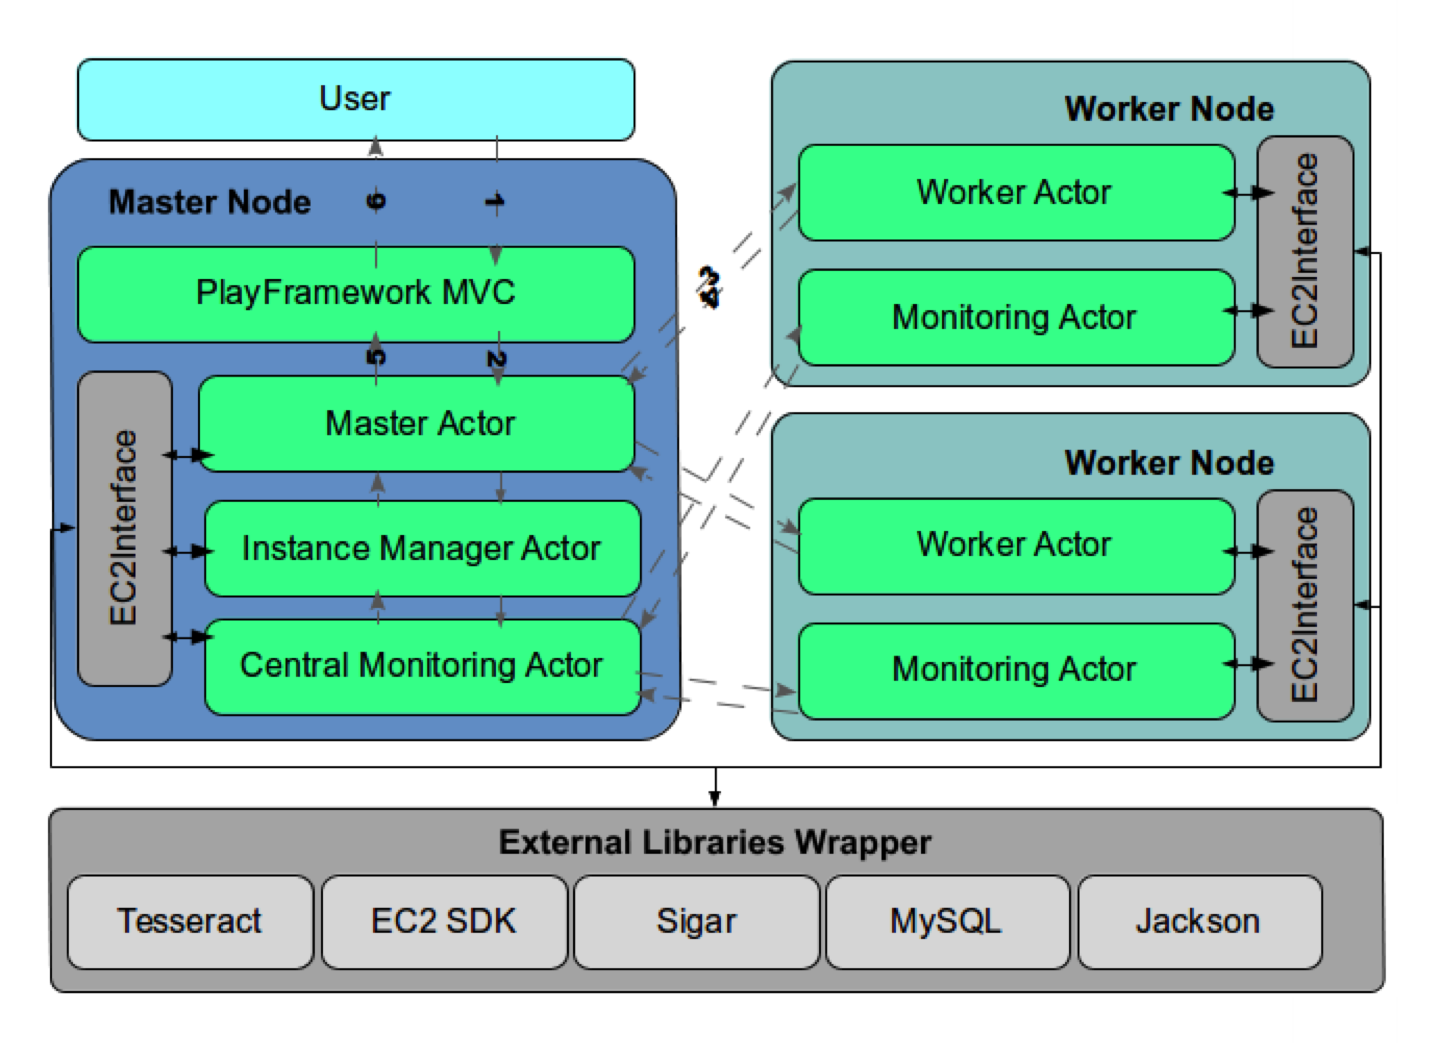
\includegraphics[totalheight=8cm,width=\linewidth]{architecture.eps}
    \caption{System Overview}
    \label{fig:sysoverview}
\end{figure}




The implementation of the major system components and policies are explained in this section: \\


%The text below is for the experimental setup, our software can be deployed on any IaaS platform
%Awsseract is designed to be deployed in Amazon EC2 [?], running on multiple EC2 Instances with Ubuntu 12.04 TLS [?] pre-installed. Typically one of these instance is in Master mode, and the rest is in Worker mode.
% Add emphaize on policy to make it easy to locate in the paragraphs
\subsubsection{Task Processing Components}\label{sec:sysdesign_task}
% First-Come, First-Served (FCFS) Policy
The Master Actor System is the main head component of the system. The Master maintains a priority queue for waiting tasks and a list of available worker actors. The Master Actor has two interfaces: receive tasks from user and send tasks for requesting workers. For the latter interface, the Master Actor receives messages for registration(authorization of worker),task request and task completion or failure from Worker Actors. The Master Actor only replies with a task from the FIFO queue if and only if a worker makes a request. If a failure is reported from the Worker, the task is put on the queue again. A difference from the Work-Stealing pattern, the Master informs Idle Workers once a task is received and put in the queue. The main reason for doing this is to avoid having a mechanism that e.g every 1 min informs the Master that the Worker is Idle so that the Worker only informs once that it is idle. This avoids a message overhead to keep informed about the worker state. However, this means that we cannot be sure if the Worker is still idle at a later point if the Master decides to send a task at a later stage (We don't have an accurate Global state of the system). Therefore, the master sends a message to inform idle workers that work is available and thus the workers that are idle will reply for work and those who reported idle earlier and are busy won't reply. 
Tasks are submitted from the web front-end developed using the Play! Framework\footnote{\url{http://www.playframework.com/}} and queued at the Master Actor.  The front-end is based on Twitter Bootstrap\footnote{\url{http://getbootstrap.com/}} and Bootswatch Amelia theme\footnote{\url{http://bootswatch.com/amelia/}} for a responsive and user-friendly design. Users are able to submit tasks using the drag-and-drop javascript library dropzone.js\footnote{\url{http://www.dropzonejs.com/}}. There is an end-user policy where users are only allowed to submit 10 tasks per day for free, while premium users has unlimited access. Both the front-end and the Master Actor System is one node in the system, named the ``Master Node". \\
% (Warning: rewriting required, memory is an issue when too many images are stored in master)
% Write in "Future Work" that priority queue is not implemented
The Worker Actor System is responsible for processing image file task using the Tesseract OCR Engine to extract the textual information. The Worker Actor has two transitional states: Working or idle. It starts first as an Idle worker and registers with the Master Actor as well as requesting for work. Once a task is received from the Master, the worker move from the Idle state to the Working state. At task completion or failure, the Worker Actor sends the results to the master and moves to Idle state. The Worker Actor system is part of the Worker node in the system. \\

The One-Master-Many-Workers design pattern let the one Master be in charge of task management and the many Workers be in charge of task execution. The minimum makespan is guaranteed by assigning the first available Worker to the oldest task. Therefore the performance requirement of the system is satisfied by fully utilizing all available Workers. \\

\subsubsection{Monitoring/Logging Components}\label{sec:sysdesign_monitor}

The Monitoring of the resources is achieved by having a Central Monitoring Actor System at the Master Node to gather and store information about System usage information from the Worker Nodes. Each Worker Node has a Monitor Actor System that every 120 seconds collect CPU, memory, and disk usage by using the Sigar Library\footnote{\url{https://support.hyperic.com/display/SIGAR/Home}}, a third-party resource monitoring library. The information is encapsulated in JSON format and sent to the Master Monitoring System. The Master Monitoring System stores the information in a SQL Database. Typically, database transactions are a bottle neck. However, the Master Monitoring Actor operates asynchronously from other Actors and does not effect the overall performance of the system. \\

The Central Monitoring Actor and Monitoring Actors together provide a complete overview of the system resource usage distribution and therefore satisfy the monitoring requirement. Furthermore, the task history and resource usage history are logged into database for further analysis. \\

%You can fix this Wing, with accurate description, even though we dont use the system info, we can mention in future work that this will be impl.
% Faulty intances should be informed from the monitoring actor i think, i have removed this part from here
\subsubsection{Instance Management Components}\label{sec:sysdesign_instance}
The Instance Manager Actor System is deployed on the Master Node and is responsible for scaling up and down depending on current user demand. This actor will shutdown(or stop) and start VMs using factors such as system usage information gathered from the Monitoring and queue information from the Master Actor System. This Management Component can be extended using Machine Learning algorithms and other means to optimize the elasticity of the system. The current implementable algorithms:  \\

\begin{itemize}
  \item \textbf{Length of the Queue:} The Instance Manager Actor set a threshold $\mathbb{L}$ on the length of the task queue and consults the Master Actor every 600 seconds to verify whether the threshold is exceeded. If so, then a new Worker Instance will be started. If the threshold $\mathbb{L}$ is not exceeded, then the Instance Manager Actor will verify whether the number of Worker Actor that is in Idle state exceeded threshold $\mathbb{I}$. If so, then some Worker Node hosting these idle Worker Actors will be stopped.
  \item \textbf{System usage information:} Instance Manager Actor consults every 600 seconds the Central Monitoring Actor whether all Worker Actors has reported their system status in the past 600 seconds. If not, the Worker Node hosting the Worker Actor is assumed to be faulty and will be stopped. \\
\end{itemize} 


\subsubsection{Libraries and Frameworks}\label{sec:sysdesign_lib}
 Awsseract utilizies several third-party libraries and frameworks. Most of the functionalities are encapsulated by a customized library wrapper EC2Interface for usage on Amazon EC2 platform. The EC2Interface provides a set of easy-to-use, tailor-made APIs that can be consumed by the different Actor Systems. The main motivation behind this implementation is not performance but to enforce a separation between the Awsseract core system and third-party libraries. This strategy allows us to only make changes inside the library wrapper without effecting the core system and deploy the system on other IaaS platforms. A summary of the libraries and frameworks used in Awsseract is presented in Table II. \\

\begin{savenotes}
\begin{table}
\renewcommand{\arraystretch}{1.3}
\caption{Libraries and Framworks}\label{tab:syslib}
\centering
\begin{tabular*}{8cm}{c|p{5cm}}
    \hline
    $Library$&$Description$\\
    \hline
    Tesseract OCR \cite{tess} & converting image file to textual information. \\
    Amaxon EC2 SDK\footnote{\url{http://aws.amazon.com/sdkforjava/}}& configuring the EC2 environment, starting and stopping instances. \\
    Sigar & collecting resources usage information of a EC2 instance. \\
    MySQL  & logging task history and resources usage history. \\
    Jackson\footnote{\url{http://jackson.codehaus.org/}}  & converting message into json string. \\
    Play! Framework & Front-end web application \\
    Akka 2.2.3 \footnote{\url{http://doc.akka.io/api/akka/2.2.3/}} & Actor\&Remote Actor Library \\

    \hline
\end{tabular*}
\end{table}
\end{savenotes}

\subsection{Additional System Features}
\noindent
Derived from Section II and III. The main additional features are presented below:

\begin{itemize}
  \item \textbf{Scheduling:} The usage of work-stealing pattern, redundancy of workers and workers report failures and restarts at runtime-related errors makes the system cost-effective and reliable
  \item \textbf{Durability:} The monitoring component saves the state of task and system usage resources in a SQL database for future analysis.  
\end{itemize} 

There are some features such as User-Profiling and Security that are present in the system. However, those features are considered for future work or a few functionalities are implemented.  

\section{Experiments}\label{sec:experiment}

\subsection{Experimental Setup}\label{sec:experimentsetup}
The set of experiments was conducted on the Amazon EC2 IaaS platform in US West (Northern California) region using the free-tier service \cite{ec2node}. The same type of hardware configuration was used for both Master and Worker nodes. A summary of the Hardware and Software configuration is presented in Table III.

\begin{table}[H]
\renewcommand{\arraystretch}{1.3}
\caption{Amazon EC2 Node Configuration}\label{tab:ec2node}
\centering
\begin{tabular*}{8cm}{c|p{5cm}}
    \hline
    $Type$&$value$\\
    \hline
    Instance type & \texttt{t1.micro} (Free-Tier) \\
    Architecture & 64-bit \\
    vCPU & 1 \\
    ECU & Variable \\
    Memory & 615 MB \\
    OS & Ubuntu Server 12.04 LTS \\
    Software & Java, Tesseract \& Scala Build Tool (sbt) \\
    \hline
\end{tabular*}
\end{table}

In total, the following 3 experiments were conducted on Amazon EC2 to verify the elasticity requirement of Asseract. In each of the experiments, a TestClient instance is set up to simulate the client machine which sends 10000 user requests to the Master instance.


\begin{itemize}
  \item \textbf{Experiment 1:} 1 Master, 1 single Worker
  \item \textbf{Experiment 2:} 1 Master, 5 static Workers
  \item \textbf{Experiment 3:} 1 Master, 1-5 dynamic Workers \\
\end{itemize} 

The first experiment verifies the successful implementation of the master-worker architecture using Akka. It also determines the baseline performance of Asseract using only 1 single Worker instance. Then the second experiment verifies the scalability of Asseract by running 5 Worker instances concurrently for load balancing. Finally, the third experiment verifies that Asseract is elastic. A very naive instance policy is applied here: If in average there are more than 500 tasks per Worker instance pending in the task queue, then a new instance is added every 10 minutes. If more than 2/3 Worker instances are idle, then terminate one Worker every 10 minutes.

\begin{figure}[H]
\centering
        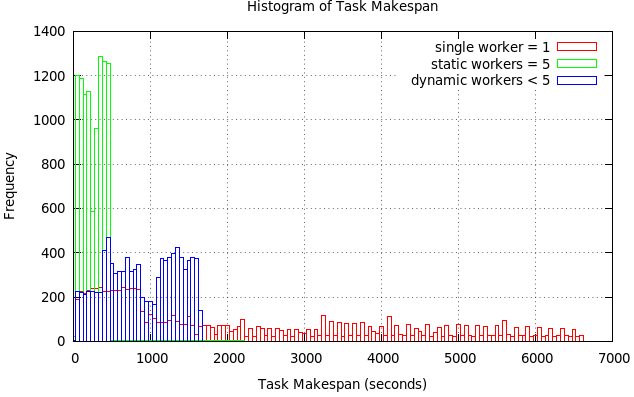
\includegraphics[totalheight=6cm,width=\linewidth]{makespan.png}
    \caption{Histogram of Task Makespan}
    \label{fig:makespan}
\end{figure}

\subsection{Experiment Results}\label{sec:experimentresults}
The logging data were retrieved from MySQL database in the Master instance, which can be found in our repository. The TaskInfo captures the lifecycle of each task and in the same way the InstanceInfo demonstrates the instance usage of Asseract.

\subsubsection{Comparison in Task Makespan}\label{sec:comparisonmakespan}
For each Task, four specific timestamps of the Task, namely the receive time, the transfer time, the start time and the finish time are logged into the database as TaskInfo. From these timestamps, the following information can be derived:

\begin{itemize}
  \item makespan = finish time - receive time
  \item queue time = transfer time - receive time
  \item transfer time = start time - transfer time
  \item processing time = finish time - start time \\
\end{itemize} 

Figure~\ref{fig:makespan} shows how the makespan of 10000 tasks changes in different experiments. When 1 Worker is deployed, it takes almost two hours to complete all tasks. When 5 static Workers are deployed, it takes only 10 minutes. This result is unfortunately even higher than the possible theoretical speedup, which seems to be caused by the uneven, unpredictable performance of Amazon EC2. Nonetheless, the experiment results verify that when more Worker Machines are deployed, the shorter the makespan. When 1-5 dynamic workers are deployed, it takes 30 minutes to complete all tasks. This result is within expectation.

\begin{table}[H]
\renewcommand{\arraystretch}{1.3}
\caption{Life Cycle of Tasks}\label{tab:tasks}
\centering
\begin{tabular*}{8cm}{c|p{1.5cm}|p{1.5cm}|p{1.5cm}}
    \hline
    & Experiment1 & Experiment2 & Experiment3\\
    \hline
    Processing Time&[0, 4]&[0, 2]&[0, 3]\\
    Transfer Time&[-1, 1]&[-1, 1]&[0, 1]\\
	Queue Time&[17,6649]&[0, 3966]&[5,1674]\\
    \hline
\end{tabular*}
\end{table}

A deeper analysis is done to verify the actual reasons behind the makespan reduction. Table  ~\ref{tab:tasks} shows that the duration of the processing time and the transfer time are relatively short (within a few seconds), that it even returns inaccurate results (negative duration is impossible). The queue time of a task depends on how fast the tasks before it are being transferred and processed, which can be reduced significantly if these tasks are processed concurrently in multiple Worker Instance. Figure~\ref{fig:queuetime} shows that the queue time distribution is almost identical to the makespan distribution, which proves that the Asseract architecture reduces makespan by decreasing the average time that a task stays in the task queue. 

\begin{figure}[H]
\centering
        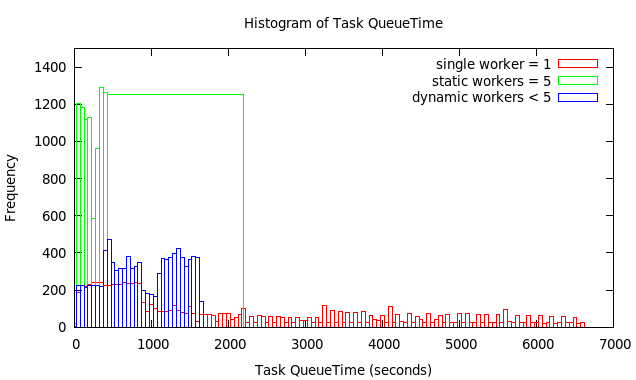
\includegraphics[totalheight=6cm,width=\linewidth]{queuetime.png}
    \caption{Histogram of Task QueueTime}
    \label{fig:queuetime}
\end{figure}

\subsubsection{Comparison in Instance Usage}\label{sec:comparisoninstance}
For each instance that was started, the start time and the stop time are logged into database as InstanceInfo. Figure~\ref{fig:instanceusage} shows how the instance usage changes in different experiments. In experiment 1 and 2, fixed number of Worker Instances are used, therefore the instance usage is constant. In experiment 3, the instance usage is regulated by the policy defined in section~\ref{sec:experimentsetup}. Only when each Worker instance has more than 500 tasks pending, new Worker instance will be initialized. After the busy period, the number of Worker instance is reduced back to 1. The instance usage using 1-5 dynamic Worker instances is only slightly higher than using 1 static Worker instance, and much less than using 5 static Worker instances, in a two-hour base.
Therefore, the lower instance usage results in a lower total runtime cost, defined by  $\sum\nolimits_{i \in instances} (stop time_{i} - start time_{i}) * instance\ cost $. This experiment does not consider the fact that Amazon EC2 charges instance usage per hour. However, similar results can be expected in a longer timeframe and with much higher workloads.

\begin{figure}[H]
\centering
        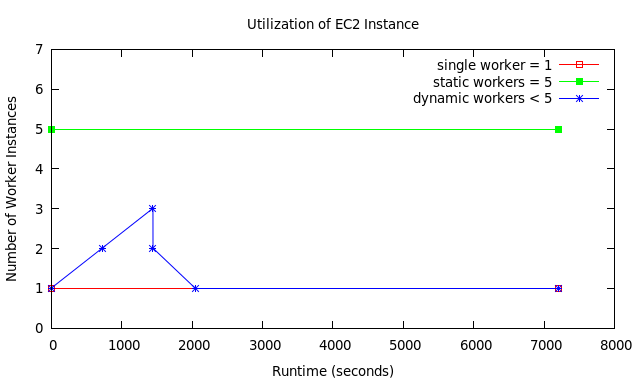
\includegraphics[totalheight=6cm,width=\linewidth]{instanceusage.png}
    \caption{Utilization of EC2 Instance}
    \label{fig:instanceusage}
\end{figure}

\subsection{Remarks on Experiment Results}\label{sec:experimentremark}
In total, 3 experiments are conducted. The first two experiments serve as baseline benchmark for the third experiment, where the actual instance policy is deployed.  In experiment 1, using one single worker results in lowest total instance cost, but longest average makespan. In experiment 2, using 5 static workers results in shortest average makespan, but highest total instance cost. Finally, in experiment 3, by assigning dynamic number of workers, the total instance cost is only slightly higher than in experiment 1, however, the average makespan is close to that of experiment 3. Furthermore, the Asseract architecture allows more sophisticated policy to be implemented, i.e. a better prediction mechanism of the workload expectation 

Although the experiments are mainly devoted for analyzing the elasticity requirement of Asseract, just by having the entire system running, the experiments also indirectly validated other system requirements specified in Table I: Asseract is able to convert a large amount of images files into textual files, with a shorter average makespan, by scheduling the workload to evenly multiple EC2 instances in a cost-efficient way.

\section{Discussion}

\section{Conclusion}
In this report, Awsseract, a prototyped distributed application on an IaaS platform, has been developed, deployed and experimented. The results shows that Awsseract deployed on the world largest IaaS Platform Amazon EC2 has high-utilization of the resources to achieve cost-effectiveness. The speed-up gained during the experiments was sub-optimal due to unoptimized parameters for scaling up. Nonetheless, many potential benefits such as no up-front commitment, elasticity, computation for relatively cheap price and ease-of-management have been shown. The main drawback with IaaS may be that confidential or organizational data may be in unsecured hands. This could potentially be solved by having confidential data on-premise and less-important on the IaaS provider. The overall verdict is that use of IaaS platform clearly meets WantCloud's current and future demands of their clients and therefore should consider using IaaS platforms to achieve better elasticity and performance. 

\bibliographystyle{plain}
\bibliography{mylib}

\section{Appendix A}
This appendix includes the time spent during implementation and experiment. 

\begin{table}[h]
\renewcommand{\arraystretch}{1.3}
\caption{Large Lab Exercise}\label{tab:exe}
\centering
\begin{tabular*}{4cm}{c|p{5cm}}
    \hline
    $Part$&$Hours$\\
    \hline
    \texttt{think-time} & 7 \\
    \texttt{dev-time} & 120 \\
    \texttt{xp-time} & 19 \\
    \texttt{analysis-time} & 5 \\
    \texttt{write-time} & 16 \\
    \texttt{wasted-time} & 6 \\
    \hline \hline
    \texttt{total-time} & 173 \\
    \hline
\end{tabular*}
\end{table}

\begin{table}[h]
\renewcommand{\arraystretch}{1.3}
\caption{Experiment }\label{tab:xp}
\centering
\begin{tabular*}{5.5cm}{c|c|c|c}
    \hline
    $Part$&$Case1$&$Case2$&$Case3$\\
    \hline
    \texttt{dev-time} &2 &2 &2  \\
    \texttt{setup-time} &3 &5 &8 \\
    \hline \hline
    \texttt{total-time} &5 &7 &10 \\
    \hline
\end{tabular*}
\end{table}


\end{document}